\section{Git}
\label{sec:git}

Today, hardly any software project is started without any form of version control system (\emph{VCS}). It supports developers as a back-up system and living archive of their work, as data generally is ephemeral and can be lost easily \cite[1]{loeliger2012version}. Although there are many different variations offered, some of the most popular ones today are \emph{Git, Apache Subversion, Mercurial} and \emph{Bazaar}.

\subsection{History}
\label{sec:git-history}
Git was initially published by \emph{Linus Torvalds} on April 7\textsuperscript{th}, 2005 \cite[6]{loeliger2012version}. This was necessary, as the ``free'' version of the then used VCS for the \emph{Linux} kernel development, \emph{BitKeeper}, was restricted in a way it was not suitable any longer for the community behind it. Furthermore, the search of an already available alternative to the BitKeeper system failed due to an unsatisfying combination of needed features, so \emph{Torvalds} came up with his own VCS flavor, containing all desired functionalities for further Linux development (among others) \cite[4]{loeliger2012version}:

\begin{itemize}
  \item Distributed development
  \item Handle thousands of developers
  \item Efficient performance
  \item Support branched development
  \item Free, as in freedom
\end{itemize}

While it was merely a tool for kernel hackers in the beginning, its simplicity quickly made developers use it for other projects too. However, the CLI still scared off people with less programming background, until GitHub came and introduced its Desktop client\footnote{\url{https://desktop.github.com/} -- GitHub Desktop client.}. Today, it is one of many GUIs, which are available for different operating systems\footnote{\url{https://git-scm.com/downloads/guis} -- Git GUI clients on the Git website.} and completely omits the necessity of terminal emulator knowledge when working with Git.

%% Write something, why it is so famous. distributed development - other use cases .. blargh.

\subsection{Technology}
\label{sec:git-technology}
Having decided to use Git as VCS, everything begins with setting up a new respository. This can be made remotely on a service like GitHub, or locally using \texttt{git init}. When initialized a local repository, it can still be published remotely through setting the correct URL using \texttt{git remote} later on \cite[198]{loeliger2012version}.

\subsubsection{Commits}
The next step would be to work with the repository. For the most part, this should not influence the developer's workflow in any way, as the \texttt{.git} directory should be automatically hidden in most modern editors to not distract him/herself from the actual work. If the developer succeeded in a sub-task or simply wanted to save the current project state, he/she would create a \emph{commit}.

A commit is a snapshot of the current repository's state. While it does not contain a copy of every file and directory in the project tree, it rather compares the current condition with its predecessing snapshot and creates a list of affected files and their changes. Blobs\footnote{\emph{BLOB} -- Binary Large OBject, a file which does not consist of queryable source code.} are either reused, if they remain unchanged or created new, if they were altered\cite[65]{loeliger2012version}.

Every commit is organized in a way, that it is chained to its predecessor (\emph{parent}), thus representing a singly linked list with the ability of gaplessly going back from the current state (\emph{head}) to the initial commit \cite[204]{dhillon2016}\cite[65]{loeliger2012version}. This is necessary, as it may happen to fix a bug or improve a design decision only by reworking a certain snapshot in the past \cite[151]{loeliger2012version}.

\subsubsection{Branches}

%% Graphic of git branches
\begin{figure} % h-ere, t-op, b-ottom, p-age
    \centering
    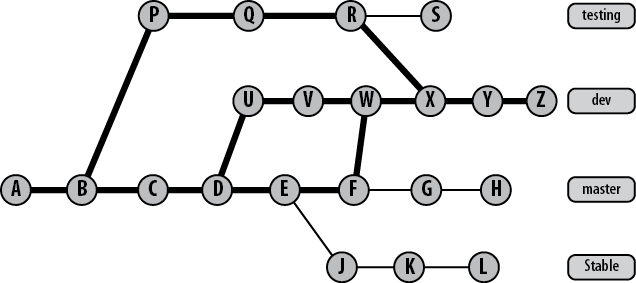
\includegraphics[width=0.8\textwidth]{git-branches.png}
    \caption{A graphic showing the basic structure of branches in Git.\\
    The \emph{testing} branch was created out of project state ``B'', whereas \emph{dev} was branched away from state ``D'' and currently holds the \emph{head commit} at ``Z''. In the meantime, \emph{testing} was merged into \emph{dev} at state ``R''. In the end, \emph{dev} contains the commit history of all states connected with the bold line \cite[p. 92f]{loeliger2012version}.}
    \label{fig:git-branches}
\end{figure}
%

Since its early days, Git was used not only as back-up or archive system, but also as code management system. This is possible due to built-in functions, such as the so-called \emph{branched development}, where a current state of the actual development is duplicated and worked on separately. It allows for development to continue in multiple directions simultaneously \cite[89]{loeliger2012version} (see Fig. \ref{fig:git-branches}).

When being part of a remote team, a developer may also \emph{push} his/her own local branches for providing it to others, as well as keeping them for local development and \emph{merging} them back to the main branch after succeeding in his current task \cite[207]{dhillon2016}. Through the use of these possibilities, a responsible administrator keeping track of the development structure is not necessarily required to be appointed in any repository settings. Furthermore, the team may decide members in charge for merges in an agile way, based on the current need.

\subsubsection{Usage in static site development}
The advantages of using Git in static site development are mainly its possibilities of providing a full-featured archive of the content and source code of each project. Seamlessly going back and forth in the website development history makes it easy to navigate between every single content edit, without loosing track of previous and future revisions. In this case, it may work significantly better than using a common database system for content storage.

Furthermore, it is also possible to make use of Git \emph{hooks}. Once a new commit is created, a hook might take care of invoking the build pipeline as a ``post-receive'' hook -- thus, the new website version gets built automatically without requiring any additional user interaction. However, hooks should be only used with caution, as they are not distributed the same way as the files tracked in a given repository and also may harm the integrity of their Git repository \cite[p. 285f]{loeliger2012version}.
